\section{Policies and Processes}\label{sec:"Policies and Processes"}
\subsection{Laws, Regulations, and Standards}
In a perfect world, there would be no laws, especially information security laws. Everyone would always do the right thing. However, the world is not perfect and we have laws and regulations that we must follow. Build your Information Security Program around these laws and regulations, not on top of them. If we only follow the letter of the law, our program will be insufficient. Your program should be structured such that it naturally meets the requirements your organization operates within. Always structure your organization to be the least regulated as possible. For example, if you only accept credit cards at two locations, segment those locations from the rest of your network. Last, these laws are usually high-level and leave the details up to you.
\begin{table}[ht]\begin{center}\begin{tabular}{|c|c|c|}\hline
\multirow{12}{.15in}{\begin{turn}{90}Information Security Program\end{turn}} &  &\multirow{6}{.15in}{\begin{turn}{270}Information Security Program\end{turn}} \\
& Laws &\\
& & \\& & \\
& Regulations &\\
& & \\
& Standards & \\
& & \\
& Policies  &\\
& Processes  &\\
& Procedures &\\
& &\\\hline
\end{tabular}\caption{Hierarchy of Governance}\end{center}\end{table}\\
Below is a list of Standards\resourcecite{WCSStandards}, Laws, and Regulations commonly encountered in the United States. All of these programs were created with the same intent: to promote good information secuirty programs. However, there are a few differences highlighted below.
Feel free to skip ahead to Policies if these seem overwhelming.\\\\
\subsubsection{Summary Table of Laws, Regulations, and Standards (Alphabet Soup)}
\begin{table}[ht]\begin{center}\begin{tabular}{ | p{2.5cm} | p{3.5cm} | p{4.5cm} | p{2cm} |}\hline
 & Industry & Sensitive Information & \\\hline
SANS & Any & Any & Guideline\\\hline
ISO & International & Any & Standard\\\hline
NIST & US & Any & Guideline\\\hline
FISMA & Federal government and contractors & Any & Law\\\hline
HIPAA & US Healthcare & EPHI & Law\\\hline
HITRUST & US Healthcare & EPHI & Standard\\\hline
PCI DSS & Credit Cards & Account Data & Regulation\\\hline
GLBA/FFIEC & Finance & Financial Information & Law\\\hline
SSAE & Third-Party Contractors & Any & Standard\\\hline
SOX & Public Companies & Any & Law\\\hline
FERPA & US Education & Student Information & Law\\\hline
NERC & North American Energy & Reliability & Regulation\\\hline
\end{tabular}\end{center}\end{table}
\subsubsection{SANS Critical Security Controls}
The SANS Critical Security Controls\resourcecite{SANSCSC} is a list of the most critical security controls from NIST SP 800-53 (discussed below).The SANS Critical Security Controls is a great place to start any Information Security Program. The list is included as Appendix: SANS Critical Security Controls - Version 5.
\subsubsection{ISO/IEC 27000-series}
ISO/IEC 27000-series\resourcecite{WISO2700} is a family of standards describing how to build and maintain an Information Security Program. It is an international standard. There are numerous modules available, and there is a cost.
\subsubsection{National Institute of Standards and Technology (NIST) Special Publications (SP) 800 Series}
The NIST SP 800 series is a collection of best practice guides for all areas of information security. These guides are the backbone of the federal government's information security programs. Many US and international organizations build their programs around these guides. Many of the concepts of these publications are discussed in this handbook. NIST SP 800-53 Revision 4:  Security and Privacy Controlsfor Federal Information Systems and Organizations\resourcecite{SP80043r4}\textsuperscript{,}\resourcecite{SP80043r4a}\textsuperscript{,}\resourcecite{W80053} is a comprehensive cata-log of security controls for U.S. federal information systems.
\subsubsection{Federal Information Security Management Act of 2002 (FISMA)}
FISMA\resourcecite{NISTFISMAIP}\textsuperscript{,}\resourcecite{WFISMA} is a federal law that requires federal agencies to create an Information Security Program based on the NIST SP 800 Series\resourcecite{NISTSP800} and focuses on the Risk Management Framework described in Risk Management. FISMA requires federal agencies to document\resourcecite{FISMAReporting} all aspects of their Information Security Program. Some federal contracts and grants require FISMA compliance for non-federal organizations. Developing a FISMA program is expensive.
\subsubsection{Health Insurance Portability and Accountability Act (HIPAA) Security Rule}
HIPAA\resourcecite{HIPAASR-P} is a federal law that regulates how Covered Entities (Healthcare Providers, Health Plans, and Health Clearinghouses) and Business Associates store, process, and transmit Electronic Protected Health Information (EPHI). HIPAA (and many other frameworks) divide information security controls into three categories: administrative, physical, and technical. These categories are often defined by the controls in them, and many controls overlap these categories. However, a technical control such as antivirus needs an administrative control to ensure it is properly installed and updated. These categories can often be helpful when framing your program. HIPAA also uses the concept of minimum necessary which is not well defined and somewhat mimics need-to-know\resourcecite{WNeedtoKnow}.
\subsubsection{Health Information Trust Alliance (HITRUST)}
HITRUST\resourcecite{HITRUST}\textsuperscript{,}\resourcecite{WHITRUST} is a three-level, healthcare-specific control framework that cross-references other Information Security Standards to simplify an organization’s compliance requirements. There is a cost.
\subsubsection{Payment Card Industry Data Security Standards (PCI DSS)} 
The PCI DSS\resourcecite{PCIDSS-P}\textsuperscript{,}\resourcecite{PCIKit} is a regulation that applies to anyone accepting credit/debit cards. It focuses on cardhard data including credit/debit card numbers.
\newpage
\begin{table}\begin{center}\begin{tabular}{ | p{5cm} | p{9cm} | }\hline
Control Objectives & PCI DSS Requirements\\\hline
Build and Maintain a Secure Network	& 1. Install and maintain a firewall configuration to protect cardholder data\\
& 2. Do not use vendor-supplied defaults for system passwords and other security parameters\\\hline
Protect Cardholder Data	& 3. Protect stored cardholder data\\
& 4. Encrypt transmission of cardholder data across open, public networks\\\hline
Maintain a Vulnerability Management Program	& 5. Use and regularly update anti-virus software on all systems commonly affected by malware\\
& 6. Develop and maintain secure systems and applications\\\hline
Implement Strong Access Control Measures & 7. Restrict access to cardholder data by business need-to-know\\
& 8. Assign a unique ID to each person with computer access\\
& 9. Restrict physical access to cardholder data\\\hline
Regularly Monitor and Test Networks & 10. Track and monitor all access to network resources and cardholder data\\
& 11. Regularly test security systems and processes\\\hline
Maintain an Information Security Policy	& 12. Maintain a policy that addresses information security\\\hline
\end{tabular}\end{center}\end{table}
\newpage
\subsubsection{Federal Financial Institutions Examination Council (FFIEC) IT Examination Handbooks}
The FFIEC regulates the financial industry through audits against their handbooks\resourcecite{FFIECBooks}. The underlying regulations protect financial information.
\subsubsection{Statement on Standards for Attestation Engagements (SSAE) 16}
SSAE 16 is a financial auditing standard that is performed by Certified Public Accountants (CPAs) against service organizations. It does not replace a Risk Assessment.
\subsubsection{Sarbanes-Oxley Act of 2002 (SOX)}
Sarbanes-Oxley Act of 2002 (SOX)\resourcecite{SOX404}
\subsubsection{Family Education Rights and Privacy Act of 1974 (FERPA; also know as the Buckley Amendment)}
\subsubsection{North American Electric Reliability Corporation (NERC)}
\subsubsection{State Laws}
\textbf{Resources}
\begin{enumerate}
\resource[WCSStandards]{Cyber Security Standards - Wikipedia}{https://en.wikipedia.org/wiki/Cyber_security_standards}
\resource[SANSCSC]{SANS Critical Security Controls}{http://www.sans.org/critical-security-controls/}
\resource[WISO2700]{ISO 27000 Series - Wikipedia}{https://en.wikipedia.org/wiki/ISO/IEC_27000-series}\
\resource[SP80043r4]{NIST Special Publication 800-53 Revision 4: Security and Privacy Controls for Federal Information Systems and Organizations}{http://nvlpubs.nist.gov/nistpubs/SpecialPublications/NIST.SP.800-53r4.pdf}
\resource[SP80043r4a]{NIST Special Publication 800-53A Revision 4: Assessing Security and Privacy Controls in Federal Information Systems and Organizations}{http://nvlpubs.nist.gov/nistpubs/SpecialPublications/NIST.SP.800-53Ar4.pdf}
\resource[W80053]{NIST Special Publication 800-53 - Wikipedia}{https://en.wikipedia.org/wiki/NIST_Special_Publication_800-53}
\resource[NISTFISMAIP]{NIST FISMA Implementation Project}{http://csrc.nist.gov/groups/SMA/fisma/index.html}
\resource[WFISMA]{Federal Information Security Management Act of 2002}{https://en.wikipedia.org/wiki/Federal_Information_Security_Management_Act_of_2002}
\resource[NISTSP800]{NIST Special Publications 800 Series}{http://csrc.nist.gov/publications/PubsSPs.html}
\resource[FISMAReporting]{FY 2010 Reporting Instructions for the Federal Information Security Management Act and Agency Privacy Management}{http://www.whitehouse.gov/sites/default/files/omb/assets/memoranda_2010/m10-15.pdf}
\resource[HIPAASR-P]{HIPAA Security Rule}{http://www.nist.gov/healthcare/security/hipaasecurity.cfm}
\resource[WNeedtoKnow]{Need to know - Wikipedia}{https://en.wikipedia.org/wiki/Need_to_know}
\resource[HITRUST]{HITRUST Alliance}{http://hitrustalliance.net}
\resource[WHITRUST]{HITRUST - Wikipedia}{https://en.wikipedia.org/wiki/HITRUST}
\resource[PCIDSS-P]{PCI DSS}{https://www.pcisecuritystandards.org/documents/PCI_DSS_v3.pdf}
\resource[PCIKit]{Open PCI Scoping Toolkit}{http://itrevolution.com/wp-content/uploads/2012/08/OpenPCIScopingToolkit.pdf}
\resource[FFIECBooks]{FFIEC IT Examination Handbook}{http://ithandbook.ffiec.gov/it-booklets.aspx}
\resource[SOX404]{SOX 404 top–down risk assessment - Wikipedia}{https://en.wikipedia.org/wiki/SOX_404_top–down_risk_assessment}
\end{enumerate}
\subsection{Policies}
Policies are the highest level of control at your organization. They help align your organization to applicable laws and regulations. Polices protect your organization, your employees, and your customers.\\\\
Because policies are created out of nothing, they require strong employee buy-in from all levels to be successful. Policy creation should involve all parts of the organization from top down and across all departments. Leadership must believe in your organization's policies, follow them, and enforce them fairly across the entire organization. This builds a strong foundation for your Information Security Program. Your policies, combined with the laws and regulations applicable to your industry, help your organization run legally and efficiently. Make vendors aware of your policies when applicable.\\\\
Policies must list consequences for non-compliance\resourcecite{WShadowIT}. Terms such as can, should, shall, and must need to be properly defined\resourcecite{RFC2119} and understood. If an employee can or should do something, does the employee have to do it?\\\\
If you need to create policies, start by documenting existing unwritten policies and processes. Many organizations download policies from SANS\resourcecite{SANSPolicies} or other organizations\resourcecite{catalyze}, change the company name, and claim they have policies. This does nothing but maybe fool an auditor. No one understands these policies or follows them. Policies templates can be useful as guides, but write your own policies that reflect your organization.\\\\
We will discuss specific policies throughout the remainder of this section and throughout this book. However, it is important to remember that policies hold the most legal strength in your organization. Employees can be fired and contracts can be terminated because of policy violations. Remember to use Plain Language when writing your policies. Review the paragraph on Plain Language in Design, Leadership, and Education and read some of the Resources in that section. To borrow terms from Creative Commons, if you write your policies in Legal English, make sure there is also a human-readable copy. For example, the SANS Dial-In Access Policy states "It is the responsibility of employees with dial-in access privileges to ensure a dial-in connection to \textless Company Name\textgreater  is not used by non-employees to gain access to company information system resources." This could also be written "Don't share your dial-in credentials." The rewritten version is shorter and clearer. This makes it more likely to be followed. However, I also wonder if anyone uses dial-up these days...
\subsection{Acceptable Use Policy}
An Acceptable Use Policy\resourcecite{WAUP}\textsuperscript{,}\resourcecite{PennAUP} clearly states the who, what, why, when, and how employees can and cannot use your organization's network and computers. This document, like all policies makes sure the employee and the organization understand the rules. All organizations need an Acceptable Use Policy.
\subsection{Information Security Policy}
Information Security Policies\resourcecite{HarvardISP}\textsuperscript{,}\resourcecite{BerkeleyMSSND} provide additional requirements for how employees use information and computers. These policies can be combined into one document or separated into several documents based on topics. Below are the most common topics covered in Information Security Policies with links to the relevant section of this book.
\subsubsection{Information Classification}
\subsubsection{Information Retention and Destruction}
\subsubsection{Change Management}
\subsubsection{Vendors}
\subsubsection{Incident Reporting and Incident Response}
\subsubsection{Disaster Recovery and Business Continuity Planning}
\subsubsection{Vulnerability Assessment and Management}
\subsubsection{Networks: Firewalls, Wireless, Remote Access}
\subsubsection{Computers: Central Management, Anti-Malware, Host-Based Firewall, Backups, etc.}
\subsubsection{Mobile Devices: Laptops, Smartphones, Mobile drives, etc.}
\subsubsection{Email, Phones, Faxes, Instant Messaging, etc.}
\subsubsection{Logs and Monitoring}
\subsubsection{Access Control: Accounts and Passwords}
\subsubsection{Encryption}
\subsubsection{Visitors}
\textbf{Resources}
\begin{enumerate}
\resource[WShadowIT]{Shadow IT - Wikipedia}{https://en.wikipedia.org/wiki/Shadow_IT}
\resource[SANSPolicies]{SANS - Information Security Policy Templates}{https://www.sans.org/security-resources/policies/}
\resource[catalyze]{Catalyze - Company Policies for HIPAA Compliance}{http://catalyzeio.github.io/policies/}
\resource[RFC2119]{RFC 2119 - Key words for use in RFCs to Indicate Requirement Levels}{http://tools.ietf.org/html/rfc2119}
\resource[WAUP]{Acceptable Use Policy - Wikipedia}{https://en.wikipedia.org/wiki/Acceptable_use_policy}
\resource[PennAUP]{Penn Computing: Policy on Acceptable Use of Electronic Resources}{http://www.upenn.edu/computing/policy/aup.html}
\resource[HarvardISP]{Harvard University - Information Security Policy}{http://policy.security.harvard.edu}
\resource[BerkeleyMSSND]{UC Berkeley - Minimum Security Standards for Networked Devices (MSSND)}{https://security.berkeley.edu/MinStds/AppA.min.htm}
\resource{An Overview of the Organizational Guidelines}{http://www.ussc.gov/sites/default/files/pdf/training/organizational-guidelines/ORGOVERVIEW.pdf}
\end{enumerate}
\subsection{Processes (and Procedures, and Standards, and Guidelines)}
Processes, Procedures, Standards, and Guidelines provide structure to your Information Security Program and help to standardize work.
\subsection{Life Cycles}\label{subsubsec:"Computer Lifecycle"}
People have a life cycle: birth, childhood, adulthood, and death. Information also has a life cycle. Networks, computers, applications, employees, and vendors have a life cycle. A generic life cycle is:
\begin{enumerate}
\item Proposal
\item Review
\item Approve
\item Implement
\item Maintain
\item Sunset
\end{enumerate}
In other words, buy something, set it up, use it, and get rid of it. The details of this process is different at each organization, but the key elements are the same.\\\\
Integrate your Information Security Program into the appropriate steps of your organization's life cycles. Consult the business owner during the proposal. Conduct an assessment including a risk assessment and a questionnaire during the review. Also classification information. Require leadership approval before implementation. Run your computer hardening process or network device hardening process during implementation. These are discussed later in this section. Also, add the item to your applicable inventory. Conduct periodic assessments as maintenance. Properly dispose of items during sunsetting.\\\\
Document your organization's life cycles and educate your employees on your organization's life cycles.
\subsection{Employee Life Cycle}\label{subsec:"Employee Life Cycle"}
There are many different job roles with different interests that interact with information security. For example, at a hospital we have
\begin{itemize}
\item Doctors and nurses who provide care for patients. They are heavy users of information,
\item Information Technology who enables the hospital to operate. They like to do cool things with fun toys,
\item Finance and administration who try to reduce cost,
\item Lawyers who reduce legal liability at the hospital,
\item And many other job roles with their own interests.
\end{itemize}
All these interests are often in conflict with each other. We sometimes call these conflicts politics or bureaucracy. However, they can all be calculated with risk.\\\\
People are your organization's most important information security control. All your employees are critical to protecting your information from attackers. Employees use information security controls all day, every day. They are also blamed for breaches. However, each failure of an employee protecting information is a failure of your information security program. Did your program educate the employee peoperly? Did your organization provide the employee with the proper resources? Evaluate the roles of employees within the context of an employee life cycle: 
\begin{itemize}
\item Onboarding
\item Ongoing
\item Offboarding
\end{itemize} We are using the term employee, but these concepts apply to anyone who works in or for your organization including contractors, volunteers, temporary staff, etc.
\subsubsection{Onboarding}
The onboarding process is everything from creating a job requisition through an employee's initial training. Begin by including including information security in job descriptions where appropriate. Consider requiring and paying for security certifications for certain positions. Everyone from information security analysts to receptions to janitors has a responsibility for information security. Make sure you hire people who have the proper experience and understand security. Ask about information security concepts during job interviews.\\\\
Many industries require various background checks (criminal, civil, and other) and reference checks. In other industries, these are a good idea. Other organizations shy away from these checks. Implement the appropriate checks for your organization and industry.\\\\
Introduce your Information Security Program to all employees at orientation. This is the beginning of your education program for each employee. Continue educating employees at orientation and throughout their employment.
Some organizations ask their coworkers to complete an attestation if they have access to sensitive information or not. If they do not work with sensitive information, they may be able to forgo the some of the requirements of your security program.
\subsubsection{Ongoing}
A great start goes a long way for introducing your employees to your information security program and company culture. However, you also need constant reinforcement. Continue your education program with periodic (weekly, monthly, yearly, etc.) education.
\subsubsection{Offboarding}
The offboarding process is the conclusion of the employee life cycle. Employees leave organizations voluntarily and involuntarily. The offboarding process should for both situations must contain the same elements in both situations. Remind the employee of his or her responsibilities and retrieve information that is the property of the organization from the employee.
\subsection{Vendor Life Cycle}
Vendors, contractors, service providers, business associates. Whatever you call them, these organizations contract with your organization to perform a service. Anytime you provide your information or access to your information to an outside organization your must perform due diligence. Due diligence means you evaluate the risks of doing business with the outside organization and mitigate those risks. We will look at the vendor life cycle similar to the employee life cycle: contracting, ongoing due diligence, and contract termination.\\\\
Everyone is excited about Cloud Computing (Infrastructure as a Service, Platform as a Service, and Software as a Service). However, Cloud Computing is nothing new to  information security. We have been contracting with these services for decades.
\subsubsection{Contracting}
Follow your purchasing process and have your purchasing, legal, risk management, intellectual property, etc. departments review the contract. Many organizations add specific language to any contract where the vendor will have access to sensitive information. These requirements could include conditions for access to the information, acceptable locations for access and storage of information (i.e. no offshoring), requirements for notifications of a breach, requirements for deletion of information when the contract is terminated, etc. Again, your purchasing and/or legal departments should help you with contracts.\\\\
Conduct an assessment of each vendor before signing a contract. This assessment could be as simple as a short questionnaire, or it could involve all the topics covered under Assessments. Several example questionnaires are included in Resources. Some vendors have prepared answers for standard questionnaires.\\\\
Some organizations require vendor's employees who will have access to sensitive information to sign the organization's acceptable use policy or a specially created document. Again, ask for this before the contract is signed.\\\\
Many organizations will often make claims such as HIPAA-compliant or SAS-70 compliant. These are not a substitute for your due diligence. FedRamp is an interesting new federal program where one federal department can sponsor the due diligence effort for a vendor and then other departments can use that same effort. This will hopefully reduce some of the duplication required for government contracts.
Please see \hyperref[subsubsec:"Business Associate Agreements"]{Business Associate Agreements} below for specific requirements in the healthcare industry.
Vendor Questionnaire organized the same as this book. Go through the Table of Contents and think about the questions that you want to ask the vendor. All organizations are different and will ask different questions. Many vendors have prepared statements about their Information Security controls that could be used in place of a questionnaire. May have one questionnaire for all vendors. May have different questionnaires for externally-hosted application, internally-hosted application, other, etc.
\subsubsection{Business Associate Agreements}\label{subsubsec:"Business Associate Agreements"}
If you work at a healthcare organization, you should be familiar with business associate agreements. These agreements must be in place with any business associates. If you are not a healthcare organization, ignore this section.
\subsubsection{Ongoing Due Diligence}
Once your organization and the vendor have singed a contract, you must continue your due diligence. Periodically reassess each vendor.
\subsubsection{Contract termination}
Similar to when you terminate an employer-employee relationship, make sure the terms of the contract are followed when you terminate it. If the contract states the vendor must delete all copies of your data, verify this has happened.\\\\
\textbf{Assessment}
\begin{description}
\item Verify you have a signed Business Associate Agreement on file for all Business Associates.
\end{description}
\textbf{Documentation}
\begin{description}
\ditem{Business Associate Agreement}
\ditem{Business Associate Policy}
\end{description}
\textbf{Risk Management}\\\\
\begin{tabularx}{\textwidth}{ X | X }
Threats & Controls \\
\hline
\tcitem{Information Security Risk at a Business Associate}{Business Associate Agreement}
\end{tabularx}\vspace{5mm}
\tccite{Information Security Risk at a Business Associate}{Business Associate Agreement}
\textbf{Resources}
\begin{enumerate}
\resource[]{Practical Measurement Framework for Software Assurance and Information Security}{https://buildsecurityin.us-cert.gov/sites/default/files/SwA_Measurement.pdf}
\resource[]{ISO 27002 Security Benchmark}{https://nigesecurityguy.wordpress.com/2013/05/28/iso-27002-security-benchmark/}
\resource[]{Information Security Program Assessment Tool}{http://www.educause.edu/library/resources/information-security-program-assessment-tool}
\resource[]{Information Security Risk Assessment Checklist}{http://www.cio.ca.gov/OIS/Government/documents/docs/RA_Checklist.doc}
\resource[]{CSA Security, Trust \& Assurance Registry}{https://cloudsecurityalliance.org/star/}
\resource[]{Consensus Assessments Initiative Questionnaire v3.0.1}{https://cloudsecurityalliance.org/download/consensus-assessments-initiative-questionnaire-v3-0-1/}
\resource[]{Business Associate Contracts}{http://www.hhs.gov/ocr/privacy/hipaa/understanding/coveredentities/contractprov.html}
\end{enumerate}
\subsection{Inventories}
Inventory document information and where it processed, stored, and transmitted.
\subsubsection{Information}
Use Data Flow Diagrams, discussed in Your First Day, to help inventory your information. Some Data Loss Prevention (DLP) products claim to inventory all your information.
\subsubsection{Networks and Computers}
Inventory your networks, network devices, and computers. Use directory services (Active Directory), DNS, and DHCP to keep records. Scan the network to verify your inventories. Optionally, keep manual inventories. Ensure inventories are up-to-date.
\subsubsection{Media}
\subsubsection{Applications}
\subsubsection{Vendors}
\textbf{Resources}
\begin{enumerate}
\resource{Visa Global Registry of Service Provider}{http://www.visa.com/splisting/searchGrsp.do}
\end{enumerate}
\subsubsection{Inventory Examples}
\begin{landscape}
\begin{table}[h]\begin{center}\begin{tabular}{|l|l|l|l|l|l|l|l|}\multicolumn{8}{l}{\textbf{Computer Inventory}}\\\hline
\parbox[t]{1cm}{Employee} & \parbox[t]{2.5cm}{Type} & \parbox[t]{1cm}{Model} & \parbox[t]{3cm}{Serial Number} & \parbox[t]{2.5cm}{Security Zone} & \parbox[t]{2cm}{Encryption} & \parbox[t]{2cm}{IP Address} & \parbox[t]{1cm}{Hostname}\\\hline
Jane Smith & Laptop & MacBook Pro & ABCD1234 & Private & FileVault 2 & DHCP & LTJaneSmith\\\hline
John Smith & Desktop & Mac Pro & ABCE1234 & Private & FileVault 2 & 10.1.1.3 & DTJohnSmith\\\hline
...&...&...&...&...&...&...&...\\\hline
\end{tabular}\end{center}\end{table}
\begin{table}[h]\begin{center}\begin{tabular}{|l|l|l|l|l|l|}\multicolumn{6}{l}{\textbf{Media Inventory}}\\\hline
\parbox[t]{1cm}{Employee} & \parbox[t]{2.5cm}{Media Type} & \parbox[t]{1cm}{Model} & \parbox[t]{3cm}{Serial Number} & \parbox[t]{4cm}{Private Information} & \parbox[t]{1cm}{Encryption}\\\hline
Jane Smith & Flash Drive & Ironkey 2GB & 1234ABCD & Allowed & Hardware AES\\\hline
John Smith & Flash Drive & Ironkey 2GB & 1235ABCD & Allowed & Hardware AES\\\hline
...&...&...&...&...&...\\\hline
\end{tabular}\end{center}\end{table}
\begin{table}[ht]\begin{center}\begin{tabular}{|l|l|l|l|l|l|l|l|}\multicolumn{8}{l}{\textbf{Application Inventory}}\\\hline
\parbox[t]{1cm}{Vendor\\Name} & \parbox[t]{1cm}{Product\\Name} & \ \parbox[t]{1.5cm}{Service\\Function} & \parbox[t]{2cm}{Maximum\\Allowed\\Downtime} & \parbox[t]{2cm}{Private\\Information} & Servers & \parbox[t]{1.6cm}{Business\\Owner} & \parbox[t]{1.6cm}{Technical\\Owner}\\\hline
Microsoft & Exchange & Email & 1 hour & Yes & \parbox[t]{3.5cm}{email.example.com (10.1.1.1)\\email2.example.com (10.1.1.2)} & \parbox[t]{1.6cm}{Jane Smith\\(CIO)} & \parbox[t]{1.6cm}{John Smith\\(CTO)} \\\hline
Microsoft & Windows & OS & N/A & Yes & N/A & \parbox[t]{1.6cm}{Jane Smith\\(CIO)} & \parbox[t]{1.6cm}{John Smith\\(CTO)} \\\hline
Microsoft & Office & \parbox[t]{1cm}{Office\\Suite} & N/A & Yes & N/A & \parbox[t]{1.6cm}{Jane Smith\\(CIO)} & \parbox[t]{1.6cm}{John Smith\\(CTO)} \\\hline
Epic & Hyperspace & EHR & 1 hour & Yes & \parbox[t]{3.5cm}{epic1.example.com (10.2.1.1)\\epic2.example.com (10.2.1.2)} & \parbox[t]{1.6cm}{Jane Smith\\(CIO)} & \parbox[t]{1.6cm}{John Smith\\(CTO)} \\\hline
... &...&...&...&...&...&...&...\\\hline
\end{tabular}\end{center}\end{table}
\begin{table}[h]\begin{center}\begin{tabular}{|l|l|l|l|l|l|l|l|l|}\multicolumn{9}{l}{\textbf{Vendor Inventory}}\\\hline
\parbox[t]{1cm}{Vendor\\Name} & \parbox[t]{1cm}{Product\\Name} & \parbox[t]{2cm}{Vendor\\Access\\to Private\\Information} & \parbox[t]{1.5cm}{Contract\\Signed} & \parbox[t]{2cm}{Business\\Associate\\Agreement\\Signed} & \parbox[t]{2cm}{Vendor Risk\\Assessment\\Completed} & \parbox[t]{1.6cm}{Business\\Owner} & \parbox[t]{1.6cm}{Technical\\Owner} & \parbox[t]{3.2cm}{Vendor\\Contact}\\\hline
Microsoft & Exchange & No & 1/1/2015 & No & No & \parbox[t]{1.6cm}{Jane Smith\\(CIO)} & \parbox[t]{1.6cm}{John Smith\\(CTO)} & \parbox[t]{3.2cm}{Jake Smith\\jake@example.com}\\\hline
Microsoft & Windows & No & 1/1/2015 & No & No & \parbox[t]{1.6cm}{Jane Smith\\(CIO)} & \parbox[t]{1.6cm}{John Smith\\(CTO)} & \parbox[t]{3.2cm}{Jake Smith\\jake@example.com}\\\hline
Microsoft & Office & No & 1/1/2015 & No & No & \parbox[t]{1.6cm}{Jane Smith\\(CIO)} & \parbox[t]{1.6cm}{John Smith\\(CTO)} & \parbox[t]{3.2cm}{Jake Smith\\jake@example.com}\\\hline
Epic & Hyperspace & Yes & 1/1/2015 & 1/1/2015 & 1/1/2015 & \parbox[t]{1.6cm}{Jane Smith\\(CIO)} & \parbox[t]{1.6cm}{John Smith\\(CTO)} & \parbox[t]{3.2cm}{Jon Smith\\jon@example.com}\\\hline
... &...&...&...&...&...&...&...&...\\\hline
\end{tabular}\end{center}\end{table}
\end{landscape}
\subsection{Disposal and Retention}\label{subsec:"Disposal and Retention"}
Information is stored on different types of media. Securely dispose of any media that possibly contains sensitive. Assume that all media contains sensitive information. Some laws or regulations mandate minimum retention periods. For example, HIPAA requires you to keep audit logs of access to PHI for 6 years. Also consider retaining logs for use in investigations.
\subsubsection{Paper Media}
Paper is a common medium for sensitive information. It is easily lost or disposed of improperly in regular trash cans. When possible, limit the amount of sensitive information stored on paper. Paper can be securely disposed of in shred bins or cross-cut shredders.\\\\
\textbf{Shred bins} are locked containers with a slot for documents. A vendor provides the bins and regularly collects the bins and destroys the contents. Place shred bins in convenient locations close to trash cans wherever possible. Place education about proper disposal around the bins and trash cans.\\\\
\textbf{Cross-cut shredders} destroy paper by cutting it into tiny pieces. They can be time consuming for large amounts of paper and are more difficult to use than shred bins. Use shred bins instead of shredders for easier convenience.
\subsubsection{Magnetic Media and Flash Media}
Hard drives, tapes, and floppy disks are all magnetic media. These devices store information by altering magnetic fields. These can be securely disposed of by a vendor or by overwriting random data on the media. Data can also be erased by placing a magnet next to the device (called degaussing), but this method is often unreliable. Some large organizations use shredders to physically destroy magnetic media and flash media.\\\\
Solid-state drives, USB drives, and SD cards are types of flash media. These devices store information in electrical circuits. Like magnetic media, flash media can be security disposed of by a vendor or by overwriting random data on the media.\\\\
\textbf{Vendors} collect magnetic media and flash media regularly or on demand. They will then destroy the media and provide a Certificate of Destruction. It may be possible to put magnetic media or flash in a paper shred bin or use the same vendor. They provide a Certificate of Destruction.\\\\
\textbf{Overwriting} magnetic media and flash media multiple times ensures any remnant data is completely erased. This process can be time consuming, especially for multiple devices. Various standards require different number of overwrites.
\subsubsection{Optical Media}
CDs and DVDs are optical media. Information is stored by lasers or other technology that create tiny indentations in the disc. Optical media can be securely disposed of by a vendor or physical destruction in shredders.\\\\
\textbf{Vendors} collect optical media just like paper, magnetic media, and flash media. The same company used for other destruction services may collect optical media. They provide a Certificate of Destruction.\\\\
\textbf{Shredders} physically destroy optical media similar to how cross-cut shredders destroy paper media.
\subsubsection{Hardware}
Laptop computers, desktop computers, servers, smart phones, tablets, digital cameras, digital voice recorders, and camcorders usually contain hard drives or flash storage. The disposal process should require these storage devices to be erased or destroyed before they leave the company.\\\\
Printers, scanners, copiers, and fax machines often contain hard drives or flash storage. The disposal process should check for these storage devices and erase or destroy them before they leave the company.\\\\
\textbf{Assessment}
\begin{description}
\aitem{Examine trash cans for paper and other media.}
\aitem{Ensure the disposal policy requires paper with sensitive information is securely disposed of.}
\aitem{Ensure the disposal policy requires magnetic media, flash media, and optical media is securely disposed of.}
\end{description}
\textbf{Documentation}
\begin{description}
\ditem{Create a disposal policy requiring the secure disposal of paper, magnetic media, flash media, and optical media. Educate employees on this policy.}
\ditem{Document the secure disposal of media when possible.}
\end{description}
\textbf{Risk Management}\\\\
\begin{tabularx}{\textwidth}{ X | X }
Threats & Controls \\
\hline
\tcitem{Improper disposal of paper, desktop computer, laptop computer, server, smart phone, tablet, digital camera, digital voice recorder, camcorder, printer, scanner, copier, or fax machine containing sensitive information.}{Secure disposal policy and assessments of disposal practices}
\end{tabularx}\vspace{5mm}
\textbf{Resources}
\begin{enumerate}
\resource[]{Data Erasure - Wikipedia}{https://en.wikipedia.org/wiki/Data_erasure}
\resource[]{Degaussing - Wikipedia}{https://en.wikipedia.org/wiki/Degaussing}
\resource[]{What do the HIPAA Privacy and Security Rules require of covered entities when they dispose of protected health information?}{http://www.hhs.gov/ocr/privacy/hipaa/faq/safeguards/575.html}
\resource[]{NIST Special Publication 800-88 Revision 1 Guidelines for Media Sanitization}{http://nvlpubs.nist.gov/nistpubs/SpecialPublications/NIST.SP.800-88r1.pdf}
\end{enumerate}
\subsection{Computer Hardening Process}\label{subsec:"Computer Hardening Process"}
All new computers should undergo your System Hardening Process to ensure they meet your baseline requirements prior to deployment. Here is a sample process:
\begin{mdframed}
\textbf{Computer Hardening Process}
\hrule
\begin{enumerate}
\item Change or remove default usernames and passwords.
\item Remove unnecessary software.
\item Disable or remove unnecessary services.
\item Install antivirus.
\item Install management or patching software.
\item Configure local policies.
\item Enable the host-based firewall.
\item Update all software.
\item Vulnerability scan the computer.
\item Vulnerability scan any web applications.
\item Enable Windows Event Logs or Syslog and configure a central log server.
\end{enumerate}
\end{mdframed}
\textbf{Assessment}
\begin{description}
\aitem{Verify there is a current, comprehensive System Hardening Process that is followed.}
\end{description}
\textbf{Documentation}
\begin{description}
\ditem{Computer Hardening Procedure}
\end{description}
\textbf{Risk Management}\\\\
\begin{tabularx}{\textwidth}{ X | X }
Threats & Controls \\
\hline
\tcitem{Compromise of a computer because of a default username and password, outdated software, or a vulnerability.}{All the controls described in the System Hardening Process}
\end{tabularx}\vspace{5mm}
\tccite{Compromise of a computer because of a default username and password, outdated software, or a vulnerability.}{All the controls described in the System Hardening Process}
\textbf{Resources}
\begin{enumerate}
\resource[]{CIS Benchmarks}{https://benchmarks.cisecurity.org/downloads/}
\resource[]{NIST National Checklist Program Repository}{http://web.nvd.nist.gov/view/ncp/repository}
\resource[]{Microsoft Baseline Security Analyzer}{http://technet.microsoft.com/en-us/security/cc184924}
\resource[]{Linux workstation security checklist}{https://github.com/lfit/itpol/blob/master/linux-workstation-security.md}
\resource[]{Mac OS X Security Configuration Guides}{https://www.apple.com/support/security/guides/}
\resource[]{Recommendations and Best Practices for Hardening Arch Linux}{https://wiki.archlinux.org/index.php/Security}
\resource[]{Securing Debian Manual}{https://www.debian.org/doc/manuals/securing-debian-howto/index.en.html}
\resource[]{End User Devices Security Guidance: Ubuntu 14.04 LTS}{https://www.gov.uk/government/publications/end-user-devices-security-guidance-ubuntu-1404-lts}
\resource[]{Security Guide: A Guide to Securing Fedora Linux}{https://docs.fedoraproject.org/en-US/Fedora/19/html/Security_Guide/index.html}
\end{enumerate}
\subsection{Network Device Hardening Process}\label{subsec:"Network Device Hardening Process"}
Exactly like your Computer Hardening Process for new computers, all new network devices should undergo your Network Device Hardening Process to ensure they meet your baseline requirements prior to deployment. Here is a sample process:
\begin{mdframed}
\textbf{Network Hardening Process}
\hrule
\begin{enumerate}
\item Change or remove default usernames and passwords.
\item Disable SNMP strings.
\item Enable NTP and configure NTP server.
\item Enable logging and configure central logging server.
\item Update all software.
\end{enumerate}
\end{mdframed}
\textbf{Assessment}
\begin{description}
\aitem{Verify there is a current, comprehensive Network Device Hardening Process that is followed.}
\end{description}
\textbf{Documentation}
\begin{description}
\ditem{Network Device Hardening Procedure}
\end{description}
\textbf{Risk Management}\\\\
\begin{tabularx}{\textwidth}{ X | X }
Threats & Controls \\
\hline
\tcitem{Compromise of a network device because of a default username and password, outdated software, or a vulnerability.}{All the controls described in the Network Device Hardening Process}
\end{tabularx}\vspace{5mm}
\textbf{Resources}
\begin{enumerate}
\resource[]{CIS Benchmarks}{https://benchmarks.cisecurity.org/downloads/}
\resource[]{NIST National Checklist Program Repository}{http://web.nvd.nist.gov/view/ncp/repository}
\end{enumerate}
\subsection{Incident Response Process}
Inputs: Security hardware and software (antimalware software, firewalls, intrustion detection/prevention system) and people (users, outside organizations and people)
Your Incident Response Process must be flexible enough to cover everything from malware on one computer to a subpoena for a user's email to a complete compromise. However, it must also be detailed enough to provide clear guidance is a time-sensitive and stressful situation. This process must be targeted to the sensitive information in industry. For example, a healthcare organization's Incident Response Process must focus on breaches of Protected Health Information and a PCI-regulated organization must focus on breaches of cardholder information. Many organizations choose to outsource  some or all of their Incident Response Process because of the technical complexity of the process and the possibility for legal action resulting from a breach. If you decide to outsource part of your Incident Response Process, you need clear rules for who will pay. Your organization also needs rules for when to remove a computer from the network. Here is a sample process:
\begin{mdframed}
\textbf{Incident Response Process and Global Incident Management}
\hrule
\begin{enumerate}
\item Declare and Incident Commander.
\item Document all actions taken including the person taking the action, the time of the action, and the result. Document all communications relating to the incident.
\item Involve any other areas of the organization such as Legal, Risk Management, Compliance, and/or Leadership.
\item Save any log information relating to the incident and network traffic between the suspect computer and the malicious host.
\item Verify the suspect computer does not perform any critical functions. These could include patient safety functions, critical business functions, etc. If the computer does perform critical business functions, refer to aforementioned rules regarding when to remove a computer from the network and discuss with the business owner.
\item Block network communication between the suspect computer and malicious hosts or remove/unplug the computer from the network to break communication with malicious hosts, stop any information theft, and prevent any additional attacks.
\item Preserve a copy of the computer's hard drive and memory for forensics. Options include removing the computer's hard drive, removing one drive from a RAID 1 array and replacing it, using software such as Norton Ghost or DD, or using specialized forensics tools.
\item Perform forensics on the hard drive and saved network traffic. Determine if any sensitive information was breached. Perform any required notifications to agencies or users.
\item Put a new hard drive in the computer or reformat the existing hard drive. Reinstall the operating system and rebuild the computer from scratch. Optionally you may attempt to remove all malicious software from the computer with anti-malware and anti-rootkit tools, update all software on the computer, and change all passwords stored on or accessed by users of the computer. However, this second method is not completely reliable because it is sometime impossible to completely remove the malware.
\item Rerun the System Hardening Process.
\end{enumerate}
\end{mdframed}
\newpage
\begin{mdframed}
\textbf{Electronic Evidence Chain of Custody}
\hrule
\begin{description}
\item Evidence Inventory
\end{description}
\begin{tabularx}{\textwidth}{ X | X | X | X }
Description & Manufacturer & Model Number & Serial Number \\
\hline
 &  &  & \\
\hline
 &  &  & \\
\hline
 &  &  & \\
\hline
 &  &  & \\
\hline
 &  &  & \\
\end{tabularx}
\begin{description}
\item Transfers of Custody
\end{description}
\begin{tabularx}{\textwidth}{ X | X | X | X }
Date and Time & Reason & From & To\\
\hline
 &  &  & \\
\hline
 &  &  & \\
\hline
 &  &  & \\
\hline
 &  &  & \\
\hline
 &  &  & \\
\end{tabularx}
\end{mdframed}
\textbf{Assessment}
\begin{description}
\aitem{Verify there is a current, comprehensive Incident Response Process.}
\aitem{Verify the process is followed.}
\end{description}
\textbf{Documentation}
\begin{description}
\ditem{Incident Response Process}
\end{description}
\textbf{Resources}
\begin{enumerate}
\resource[]{UC Privacy and Data Security Incident Response Plan}{http://www.ucop.edu/information-technology-services/_files/uc_incidentresp_plan.pdf}
\resource[]{NIST Special Publication 800-61 Revision 2 Computer Security Incident Handling Guide}{http://csrc.nist.gov/publications/nistpubs/800-61rev2/SP800-61rev2.pdf}
\resource[]{Privacy Rights Clearinghouse}{https://www.privacyrights.org}
\resource[]{Fact Sheet 17b: How to Deal with a Security Breach}{https://www.privacyrights.org/how-to-deal-security-breach}
\resource[]{Chain of Custody - Wikipedia}{https://en.wikipedia.org/wiki/Chain_of_custody}
\resource[]{Incident Command System - Wikipedia}{https://en.wikipedia.org/wiki/Incident_Command_System}
\resource[]{Computer Security Incident Management - Wikipedia}{https://en.wikipedia.org/wiki/Computer_security_incident_management}
\end{enumerate}
\subsection{Forensics}
Most organizations hire vendors to perform forensics for them because it is a specialized field and hopefully you don't need it often. The leading tool for forensics is Encase; however, you can do a lot without it.
\begin{figure}[h]
\centering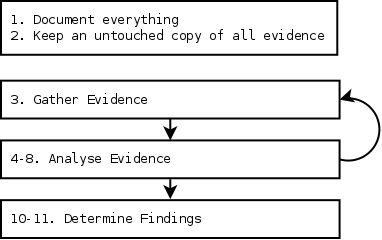
\includegraphics[scale=.75]{./img/Forensics}
\caption{Forensics}
\end{figure}
\begin{enumerate}
\item Document everything.
\item Keep an untouched copy of all evidence.
\item Gather all relevant information
\begin{itemize}
\item Disk images (including memory images) from compromised computers
\item Logs (Windows Event Logs, syslog, web server logs, web client logs, SQL server logs, Remote Desktop logs, SSH logs, etc.) from the compromised computer and other computers
\item Logs from network devices (Firewalls, Intrusion Detection Systems, Anti-malware consoles, etc.)
\item Netflow data from network devices
\end{itemize}
\item Create a calendar and add all relevant dates and times.
\item Run forensics software and a couple anti-malware programs against all disk images. 
\begin{itemize}
\item Redline \url{https://www.mandiant.com/resources/download/redline}
\item Encase \url{https://www.guidancesoftware.com}
\item \url{https://en.wikipedia.org/wiki/EnCase}
\item Please see Malware for more information on anti-malware programs.
\end{itemize}
\item Perform Malware Analysis on any malware. This is a full time job at security or large companies. Alternatively, calculate a hash of all files, and compare these hashes with malware lists.
\begin{itemize}
\item Practical Malware Analysis \url{http://www.nostarch.com/malware}
\item ThreatGRID Malware Analysis and Threat Intelligence \url{http://www.threatgrid.com}
\item National Software Reference Library \url{http://www.nsrl.nist.gov}
\end{itemize}
\item Manually and/or automatically search through the above relevant information for anything interesting. Ask your users for additional information. 
\begin{itemize}
\item Dates
\item IP addresses and URLs
\item Usernames
\item Programs and services
\item Emails
\item Files (Microsoft Office, PDFs, CSVs, etc.)
\end{itemize}
\item Check IP addresses and URLs against malware lists, location information, hostname lists, etc.
\begin{itemize}
\item IP Address Blacklist Checker Tool \url{http://www.ipvoid.com} 
\item ThreatSTOP | Check an IP address \url{http://threatstop.com/checkip}
\item MalwareURL - Website status verification \url{http://www.malwareurl.com/listing-urls.php}
\item Malware Domain List \url{http://www.malwaredomainlist.com/mdl.php}
\item IP Tracker: Lookup, Find, Track \& Trace IP Address \url{http://www.ip-tracker.org}
\item WebHosting.Info's Power WHOIS Service \url{http://whois.webhosting.info}
\end{itemize}
\item Repeat steps 3-8 as necessary.
\item Determine how the computer was compromised.
\item Determine the extent of the compromise.
\begin{itemize}
\item Were other computers compromised from this computer?
\item Was any information exfiltrated from or through this computer?
\end{itemize}
\end{enumerate}
\textbf{Resources}
\begin{enumerate}
\resource[]{Network Security Through Data Analysis}{http://shop.oreilly.com/product/0636920028444.do}
\resource[]{Forensics Wiki}{http://www.forensicswiki.org/wiki/Main_Page}
\resource[]{DD - Wikipedia}{https://en.wikipedia.org/wiki/Dd_(Unix)}
\resource[]{Autopsy}{http://www.sleuthkit.org/autopsy/}
\resource[]{Hex Editor - Wikipedia}{https://en.wikipedia.org/wiki/Hex_editor}
\resource[]{Encase}{https://www.guidancesoftware.com/products/Pages/encase-forensic/overview.aspx}
\resource[]{ProDiscover Basic}{http://www.prodiscover-basic.software.informer.com}
\end{enumerate}
\subsubsection{Malware Reverse Engineering}
\textbf{Resources}
\begin{enumerate}
\resource[]{Cuckoo Sandbox}{http://cuckoosandbox.org}
\resource[]{IDA Pro}{https://www.hex-rays.com/products/ida/index.shtml}
\end{enumerate}